% Options for packages loaded elsewhere
\PassOptionsToPackage{unicode}{hyperref}
\PassOptionsToPackage{hyphens}{url}
\PassOptionsToPackage{space}{xeCJK}
%
\documentclass[
  letterpaper,
  DIV=11,
  numbers=noendperiod,
  nottoc,
  oneside]{scrreprt}

\usepackage{amsmath,amssymb}
\usepackage{iftex}
\ifPDFTeX
  \usepackage[T1]{fontenc}
  \usepackage[utf8]{inputenc}
  \usepackage{textcomp} % provide euro and other symbols
\else % if luatex or xetex
  \usepackage{unicode-math}
  \defaultfontfeatures{Scale=MatchLowercase}
  \defaultfontfeatures[\rmfamily]{Ligatures=TeX,Scale=1}
\fi
\usepackage{lmodern}
\ifPDFTeX\else  
    % xetex/luatex font selection
    \setmainfont[]{Crimson}
  \ifXeTeX
    \usepackage{xeCJK}
    \setCJKmainfont[]{Noto Serif KR}
          \fi
  \ifLuaTeX
    \usepackage[]{luatexja-fontspec}
    \setmainjfont[]{Noto Serif KR}
  \fi
\fi
% Use upquote if available, for straight quotes in verbatim environments
\IfFileExists{upquote.sty}{\usepackage{upquote}}{}
\IfFileExists{microtype.sty}{% use microtype if available
  \usepackage[]{microtype}
  \UseMicrotypeSet[protrusion]{basicmath} % disable protrusion for tt fonts
}{}
\makeatletter
\@ifundefined{KOMAClassName}{% if non-KOMA class
  \IfFileExists{parskip.sty}{%
    \usepackage{parskip}
  }{% else
    \setlength{\parindent}{0pt}
    \setlength{\parskip}{6pt plus 2pt minus 1pt}}
}{% if KOMA class
  \KOMAoptions{parskip=half}}
\makeatother
\usepackage{xcolor}
\usepackage[left=2in,right=2in,marginparwidth=1.5in,twoside=true]{geometry}
\setlength{\emergencystretch}{3em} % prevent overfull lines
\setcounter{secnumdepth}{5}
% Make \paragraph and \subparagraph free-standing
\makeatletter
\ifx\paragraph\undefined\else
  \let\oldparagraph\paragraph
  \renewcommand{\paragraph}{
    \@ifstar
      \xxxParagraphStar
      \xxxParagraphNoStar
  }
  \newcommand{\xxxParagraphStar}[1]{\oldparagraph*{#1}\mbox{}}
  \newcommand{\xxxParagraphNoStar}[1]{\oldparagraph{#1}\mbox{}}
\fi
\ifx\subparagraph\undefined\else
  \let\oldsubparagraph\subparagraph
  \renewcommand{\subparagraph}{
    \@ifstar
      \xxxSubParagraphStar
      \xxxSubParagraphNoStar
  }
  \newcommand{\xxxSubParagraphStar}[1]{\oldsubparagraph*{#1}\mbox{}}
  \newcommand{\xxxSubParagraphNoStar}[1]{\oldsubparagraph{#1}\mbox{}}
\fi
\makeatother


\providecommand{\tightlist}{%
  \setlength{\itemsep}{0pt}\setlength{\parskip}{0pt}}\usepackage{longtable,booktabs,array}
\usepackage{calc} % for calculating minipage widths
% Correct order of tables after \paragraph or \subparagraph
\usepackage{etoolbox}
\makeatletter
\patchcmd\longtable{\par}{\if@noskipsec\mbox{}\fi\par}{}{}
\makeatother
% Allow footnotes in longtable head/foot
\IfFileExists{footnotehyper.sty}{\usepackage{footnotehyper}}{\usepackage{footnote}}
\makesavenoteenv{longtable}
\usepackage{graphicx}
\makeatletter
\def\maxwidth{\ifdim\Gin@nat@width>\linewidth\linewidth\else\Gin@nat@width\fi}
\def\maxheight{\ifdim\Gin@nat@height>\textheight\textheight\else\Gin@nat@height\fi}
\makeatother
% Scale images if necessary, so that they will not overflow the page
% margins by default, and it is still possible to overwrite the defaults
% using explicit options in \includegraphics[width, height, ...]{}
\setkeys{Gin}{width=\maxwidth,height=\maxheight,keepaspectratio}
% Set default figure placement to htbp
\makeatletter
\def\fps@figure{htbp}
\makeatother
% definitions for citeproc citations
\NewDocumentCommand\citeproctext{}{}
\NewDocumentCommand\citeproc{mm}{%
  \begingroup\def\citeproctext{#2}\cite{#1}\endgroup}
\makeatletter
 % allow citations to break across lines
 \let\@cite@ofmt\@firstofone
 % avoid brackets around text for \cite:
 \def\@biblabel#1{}
 \def\@cite#1#2{{#1\if@tempswa , #2\fi}}
\makeatother
\newlength{\cslhangindent}
\setlength{\cslhangindent}{1.5em}
\newlength{\csllabelwidth}
\setlength{\csllabelwidth}{3em}
\newenvironment{CSLReferences}[2] % #1 hanging-indent, #2 entry-spacing
 {\begin{list}{}{%
  \setlength{\itemindent}{0pt}
  \setlength{\leftmargin}{0pt}
  \setlength{\parsep}{0pt}
  % turn on hanging indent if param 1 is 1
  \ifodd #1
   \setlength{\leftmargin}{\cslhangindent}
   \setlength{\itemindent}{-1\cslhangindent}
  \fi
  % set entry spacing
  \setlength{\itemsep}{#2\baselineskip}}}
 {\end{list}}
\usepackage{calc}
\newcommand{\CSLBlock}[1]{\hfill\break\parbox[t]{\linewidth}{\strut\ignorespaces#1\strut}}
\newcommand{\CSLLeftMargin}[1]{\parbox[t]{\csllabelwidth}{\strut#1\strut}}
\newcommand{\CSLRightInline}[1]{\parbox[t]{\linewidth - \csllabelwidth}{\strut#1\strut}}
\newcommand{\CSLIndent}[1]{\hspace{\cslhangindent}#1}

\usepackage{tocbibind}  % Include TOC, List of Figures, and List of Tables in the TOC
\usepackage{fontspec}
\KOMAoption{captions}{tableheading}
\makeatletter
\@ifpackageloaded{bookmark}{}{\usepackage{bookmark}}
\makeatother
\makeatletter
\@ifpackageloaded{caption}{}{\usepackage{caption}}
\AtBeginDocument{%
\ifdefined\contentsname
  \renewcommand*\contentsname{Table of contents}
\else
  \newcommand\contentsname{Table of contents}
\fi
\ifdefined\listfigurename
  \renewcommand*\listfigurename{List of Figures}
\else
  \newcommand\listfigurename{List of Figures}
\fi
\ifdefined\listtablename
  \renewcommand*\listtablename{List of Tables}
\else
  \newcommand\listtablename{List of Tables}
\fi
\ifdefined\figurename
  \renewcommand*\figurename{Figure}
\else
  \newcommand\figurename{Figure}
\fi
\ifdefined\tablename
  \renewcommand*\tablename{Table}
\else
  \newcommand\tablename{Table}
\fi
}
\@ifpackageloaded{float}{}{\usepackage{float}}
\floatstyle{ruled}
\@ifundefined{c@chapter}{\newfloat{codelisting}{h}{lop}}{\newfloat{codelisting}{h}{lop}[chapter]}
\floatname{codelisting}{Listing}
\newcommand*\listoflistings{\listof{codelisting}{List of Listings}}
\makeatother
\makeatletter
\makeatother
\makeatletter
\@ifpackageloaded{caption}{}{\usepackage{caption}}
\@ifpackageloaded{subcaption}{}{\usepackage{subcaption}}
\makeatother
\makeatletter
\@ifpackageloaded{sidenotes}{}{\usepackage{sidenotes}}
\@ifpackageloaded{marginnote}{}{\usepackage{marginnote}}
\makeatother

\ifLuaTeX
  \usepackage{selnolig}  % disable illegal ligatures
\fi
\usepackage{bookmark}

\IfFileExists{xurl.sty}{\usepackage{xurl}}{} % add URL line breaks if available
\urlstyle{same} % disable monospaced font for URLs
\hypersetup{
  pdftitle={Multi-Word Representations in Minds and Models: Investigating Storage Mechanisms in Humans and Large Language Models},
  pdfauthor={Zachary Nicholas Houghton},
  hidelinks,
  pdfcreator={LaTeX via pandoc}}


\title{Multi-Word Representations in Minds and Models: Investigating
Storage Mechanisms in Humans and Large Language Models}
\author{Zachary Nicholas Houghton}
\date{2024-11-25}

\begin{document}
\maketitle

\pagenumbering{roman}

\renewcommand*\contentsname{Table of contents}
{
\setcounter{tocdepth}{2}
\tableofcontents
}
\listoffigures
\listoftables

\bookmarksetup{startatroot}

\chapter*{Abstract}\label{sec-abstract}
\addcontentsline{toc}{chapter}{Abstract}

\markboth{Abstract}{Abstract}

This is my abstract.

\bookmarksetup{startatroot}

\chapter*{Acknowledgements}\label{sec-acknowledgements}
\addcontentsline{toc}{chapter}{Acknowledgements}

\markboth{Acknowledgements}{Acknowledgements}

I started this journey in the middle of a pandemic that persisted
through much of my program. It is no exaggeration to say that my success
in this program is due in large, or perhaps completely, to the people
below. {\marginnote{\begin{footnotesize}Though I would like to take some
of the credit for myself.\end{footnotesize}}}

First and foremost, I would not be here if it weren't for my incredible
advisor, Dr.~Emily Morgan. Emily has been a never-ending source of
knowledge, a guiding light, and a constant source of reassurance. Emily
was charged with the non-trivial task of helping to translate my
incoherent stream of thoughts into a coherent set of ideas. She pushed
me hard, believed in me, and never let me fall behind. Words can express
neither the gratitude nor the debt that I owe to you, Emily.

I'd also like to thank many of the other brilliant minds here who have
been crucial to my development as a researcher. Specifically, I'd like
to thank Dr.~Fernanda Ferreira, Dr.~Kenji Sagae, Dr.~Santiago Barreda,
Dr.~Georgia Zellou, and Dr.~Masoud Jasbi. Over my years at UC Davis,
each of these professors has volunteered countless hours of their time
and wisdom to me, indulging my endless stream of questions.

Many of the ideas presented here have benefited in some form or another
from feedback from many brilliant graduate students. I would especially
like to thank Casey Felton, Harvey Qiu, Skyler Reese, Nicole Dodd, and
Penny Pan for their feedback on much of the work included here.

I'd also like to thank Casey, Felix, and Nora for being a strong support
system during my time here. Our Sunday shenanigans were a welcomed
escape from the tireless work of completing a PhD.

My journey in linguistics started at the University of Oregon, and I
want to thank all of the professors that supported the beginning of my
journey. I particularly want to acknowledge Dr.~Vsevolod Kapatsinski.
Volya has donated countless hours of his time to me even after his role
as my undergraduate thesis advisor was long over. He continues to be an
endless source of knowledge and inspiration and much of my knowledge and
interest in language learning comes from him. Perhaps more importantly,
however, he is a constant reminder that linguistics is \emph{fun}! Had
it not been for our meetings over the years that devolved into
ridiculous linguistic tangents, I would have burnt out long ago. I would
not be here without you, Volya.

I would also like to thank Kim 선생님. Her words of encouragement and
faith in me helped me believe in myself.

In addition, I want to thank Dr.~Melissa Baese-Berk, Dr.~Misaki Kato,
and Dr.~Zara Harmon. Aside from being both exceptional researchers and
inspirational people, each one of them was crucial to my development as
a researcher, as a linguist, and as a person. If I can become even half
the linguist they are, I'll be incredibly proud of myself.

Along with the technical and academic guidance, it also would have been
impossible to complete this PhD without the unending support I received
from my many close friends. It would take up too much space to name all
of them, but they surely know who they are.

I have been fortunate to have a strong support system in the form of of
my two sisters, Kayla and Lily. We've been through so much together. I
don't know where I would be, not just academically, but more generally
in life, had you two not been by my side.

This work would also have not been completed without the influence of my
parents. Specifically, I want to thank my mom for teaching me that the
ability to find the answer is far more important than knowing the
answer, and my dad, for teaching me the discipline and practical skills
to achieve my goals.

Finally, I would like to thank Addy, Charles, Spencer, Paul, Wyatt, and
보미 for being my very strong support network. Despite being thousands
of miles away I could always count on all of you when times were tough.

The number of people who have been indispensable in me getting here is
undoubtedly larger than is feasible to include here. To those that I
have inevitably left out, I apologize.

\bookmarksetup{startatroot}

\chapter{Introduction}\label{introduction}

\pagenumbering{arabic}

\section{Computation and Storage}\label{computation-and-storage}

From a young age, humans are capable of generating sentences that
they've never encountered before
(\citeproc{ref-kapatsinskiChangingMindsChanging2018}{Kapatsinski 2018};
\citeproc{ref-berkoChildsLearningEnglish1958}{Berko 1958}). This ability
is largely enabled by our ability to store forms that we've learned and
compute new forms by applying knowledge of the grammar to these stored
forms (\citeproc{ref-stembergerAreInflectedForms2004}{Joseph P.
Stemberger and MacWhinney 2004};
\citeproc{ref-stembergerFrequencyLexicalStorage1986}{Joseph Paul
Stemberger and MacWhinney 1986};
\citeproc{ref-morganAbstractKnowledgeDirect2016}{Morgan and Levy 2016},
\citeproc{ref-morganModelingIdiosyncraticPreferences2015}{2015};
\citeproc{ref-berkoChildsLearningEnglish1958}{Berko 1958}). In theory,
these can be complementary forces: if a form is stored, it does not need
to be computed, and if a form can be computed, it does not have to be
stored. For example, if the word \emph{cats} is stored, then there is
not necessarily a reason to compute it (e.g., by combining the lexical
root, \emph{cat}, with a general plural rule, -\emph{s}). On the other
hand, if it can be computed (e.g., we have learned the word \emph{cat},
and we have learned how to make regular forms plural in English), then
there may be no reason to store it. This has been the story told by many
of the early linguistic theories (e.g.,
\citeproc{ref-chomsky1965}{Chomsky 1965}), and understandably so.

Early theories argued for a strict division between items that are
stored and items that are computed (\citeproc{ref-chomsky1965}{Chomsky
1965}). These theories often prioritized efficiency and minimizing
memory consumption. Storing items that could be generated
computationally was considered redundant.

-What is computation? What is storage?

-Chomsky accounts (minimal storage)

-Bybeean accounts (frequent items stored)

-Evidence for storage

~ ~ ~-Evidence from phonology, learning, semantics, processing, regular
vs irregular forms

-Storage at a syllable-level, word-level, phrasal-level, and
sentence-level.

-Evidence for computation

~ ~ ~-less important to show, taken for granted, can mention
Berko-Gleason

\section{What is Storage?}\label{what-is-storage}

-What does it mean for something to be stored?

~ ~ ~-Exemplar theories

~ ~ ~-Abstractions

-What happens to stored items?~~

~ ~ ~ -How are they stored (internal structure)

~ ~ ~ -How are they processed?

~ ~ ~ -Potential competition effects~

\section{\texorpdfstring{\textbf{Models of
Storage}}{Models of Storage}}\label{models-of-storage}

-Fragment grammars

-LLMs

-What can we learn from them?

\section{\texorpdfstring{\textbf{Q}uestions}{Questions}}\label{questions}

-What drives storage?

~ ~ -Confident about frequency effects, but what about predictability?

-How are stored units processed?

~ ~ -language processing is inherently linear, how does this interact
with holistic storage?

-What happens to the internal structure of stored units?

~ ~ ~-e.g., Kapatsinski \& Radicke

\bookmarksetup{startatroot}

\chapter{staub\_replication\_and\_extension}\label{staub_replication_and_extension}

The results from our previous experiments could be a task-specific
property of the maze task, since it forces participants to make a
decision which may commit them to a specific interpretation in a way
that more naturalistic reading may not. Thus, in this Experiment we
replicate the previous experiment using eye-tracking.

\section{Methods}\label{methods}

\subsection{Participants}\label{participants}

56 native English speakers were recruited from the University of
California, Davis subjects pool. They were given course credit in
exchange for their participation. All participants had normal or
corrected vision.

\subsection{Materials}\label{materials}

The materials here were identical to those in Experiment 2.

\subsection{Procedure}\label{procedure}

We recorded participants' eye movements using the Eyelink 1000 Plus. We
recorded pupil movements from the right eye. Participants were seated
850mm away from the screen. Our screen resolution was 1920x1080, 531.3mm
in width, and 298.8mm in height.

Comprehension was checked for non-experimental trials and participants
below 80\% accuracy were excluded. Out of our 56 participants, 0 were
excluded for falling below the accuracy threshold.

\subsection{Analyses}\label{analyses}

Prior to our analyses, sentences with blinks were excluded and fixations
less than 80ms in duration and within one character of the nearest
fixation were merged into that fixation (following
\citeproc{ref-staubTimeCoursePlausibility2007}{Staub et al. 2007}). For
our regions of interest (the first noun and the second noun
independently in the compound n oun), we computed first fixation
duration, first pass time, and go-past time.

For each analysis, our independent variables were plausibility (high or
low) and (log) predictability (high or low) and their interaction. We
also included random slopes for condition and predictability by subject
and plausibility by compound noun as well as intercepts for subject and
compound noun. For each of our models, we used sum-coded, where the
intercept represents the grand mean and the fixed-effect coefficient
estimates represent the distance from the grand mean.

\section{Results}\label{results}

\subsection{First Fixation Times}\label{first-fixation-times}

\subsubsection{N1}\label{n1}

First, we examined the effects of plausibility and predictability on
first fixation times for the first noun. Note that in our case, since
plausibility was codes as -1 for plausible and 1 for implausible, a
positive coefficient estimate of plausibility corresponds to longer
fixation times for implausible items. Additionally, following Houghton
et al.
(\citeproc{ref-houghtonTaskdependentConsequencesDisfluency2024}{2024})
we also report the percentage of posterior samples greater than zero.
Our model results can be found below in Table~\ref{tbl-firstfixn1} and a
visualization can be found in Figure~\ref{fig-firstfixn1}.

\begin{longtable}[]{@{}
  >{\raggedright\arraybackslash}p{(\columnwidth - 10\tabcolsep) * \real{0.3636}}
  >{\raggedright\arraybackslash}p{(\columnwidth - 10\tabcolsep) * \real{0.1169}}
  >{\raggedright\arraybackslash}p{(\columnwidth - 10\tabcolsep) * \real{0.1299}}
  >{\raggedright\arraybackslash}p{(\columnwidth - 10\tabcolsep) * \real{0.1039}}
  >{\raggedright\arraybackslash}p{(\columnwidth - 10\tabcolsep) * \real{0.1039}}
  >{\raggedleft\arraybackslash}p{(\columnwidth - 10\tabcolsep) * \real{0.1818}}@{}}

\caption{\label{tbl-firstfixn1}Model results examining the effect of
plausibility and predictability on first fixation times for the N1
region.}

\tabularnewline

\toprule\noalign{}
\begin{minipage}[b]{\linewidth}\raggedright
\end{minipage} & \begin{minipage}[b]{\linewidth}\raggedright
Estimate
\end{minipage} & \begin{minipage}[b]{\linewidth}\raggedright
Est.Error
\end{minipage} & \begin{minipage}[b]{\linewidth}\raggedright
Q2.5
\end{minipage} & \begin{minipage}[b]{\linewidth}\raggedright
Q97.5
\end{minipage} & \begin{minipage}[b]{\linewidth}\raggedleft
\% Samples \textgreater{} 0
\end{minipage} \\
\midrule\noalign{}
\endhead
\bottomrule\noalign{}
\endlastfoot
Intercept & 231.016 & 4.433 & 222.356 & 239.502 & 100.00 \\
Plausibility & 1.661 & 2.020 & -2.289 & 5.695 & 78.95 \\
Predictability & 2.782 & 2.870 & -2.804 & 8.532 & 83.75 \\
Plausibility:Predictability & -3.473 & 2.012 & -7.418 & 0.522 & 4.15 \\

\end{longtable}

\begin{figure}

\centering{

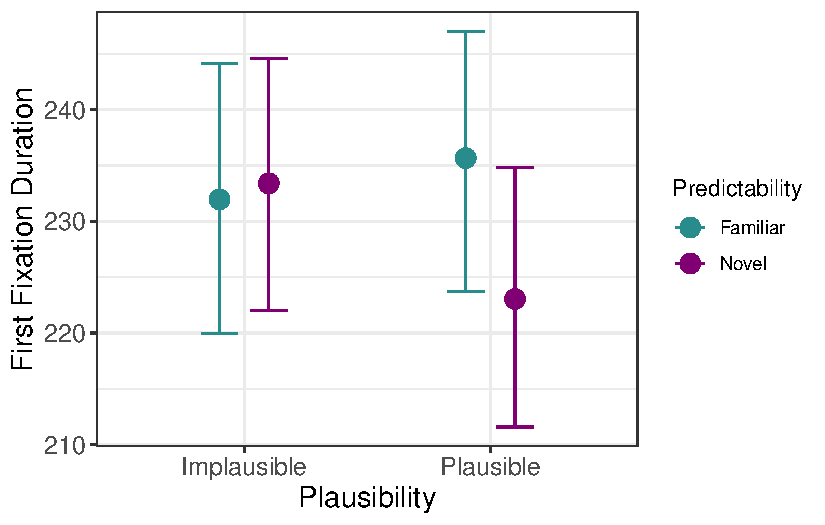
\includegraphics[width=0.8\textwidth,height=\textheight]{Chapters/Compound Nouns/staub_rep_ext_files/figure-pdf/fig-firstfixn1-1.pdf}

}

\caption{\label{fig-firstfixn1}Visualization of the effects of
plausibility and predictability on first fixation times for the N1
region.}

\end{figure}%

Our results for first-fixation times, while non-significant, do show an
interesting trend, with the effect of plausibility in the expected
direction (although with only \textasciitilde78\% samples greater than
zero). While 96\% of the samples less than zero for the interaction
effect, the effect size is so small that it's not particularly
meaningful.

\subsubsection{N2}\label{n2}

Next we examine the effects of plausibility and predictability on the
first fixation times of the second noun in the compound.

\begin{longtable}[]{@{}
  >{\raggedright\arraybackslash}p{(\columnwidth - 10\tabcolsep) * \real{0.3636}}
  >{\raggedright\arraybackslash}p{(\columnwidth - 10\tabcolsep) * \real{0.1169}}
  >{\raggedright\arraybackslash}p{(\columnwidth - 10\tabcolsep) * \real{0.1299}}
  >{\raggedright\arraybackslash}p{(\columnwidth - 10\tabcolsep) * \real{0.1039}}
  >{\raggedright\arraybackslash}p{(\columnwidth - 10\tabcolsep) * \real{0.1039}}
  >{\raggedleft\arraybackslash}p{(\columnwidth - 10\tabcolsep) * \real{0.1818}}@{}}

\caption{\label{tbl-firstfixn2}Model results examining the effect of
plausibility and predictability on first fixation times for the N2
region.}

\tabularnewline

\toprule\noalign{}
\begin{minipage}[b]{\linewidth}\raggedright
\end{minipage} & \begin{minipage}[b]{\linewidth}\raggedright
Estimate
\end{minipage} & \begin{minipage}[b]{\linewidth}\raggedright
Est.Error
\end{minipage} & \begin{minipage}[b]{\linewidth}\raggedright
Q2.5
\end{minipage} & \begin{minipage}[b]{\linewidth}\raggedright
Q97.5
\end{minipage} & \begin{minipage}[b]{\linewidth}\raggedleft
\% Samples \textgreater{} 0
\end{minipage} \\
\midrule\noalign{}
\endhead
\bottomrule\noalign{}
\endlastfoot
Intercept & 234.448 & 4.864 & 224.479 & 243.767 & 100.000 \\
Plausibility & -2.151 & 2.973 & -8.132 & 3.685 & 23.225 \\
Predictability & -4.136 & 2.988 & -9.887 & 1.887 & 8.575 \\
Plausibility:Predictability & -2.928 & 3.012 & -8.920 & 2.967 &
16.075 \\

\end{longtable}

\begin{figure}

\centering{

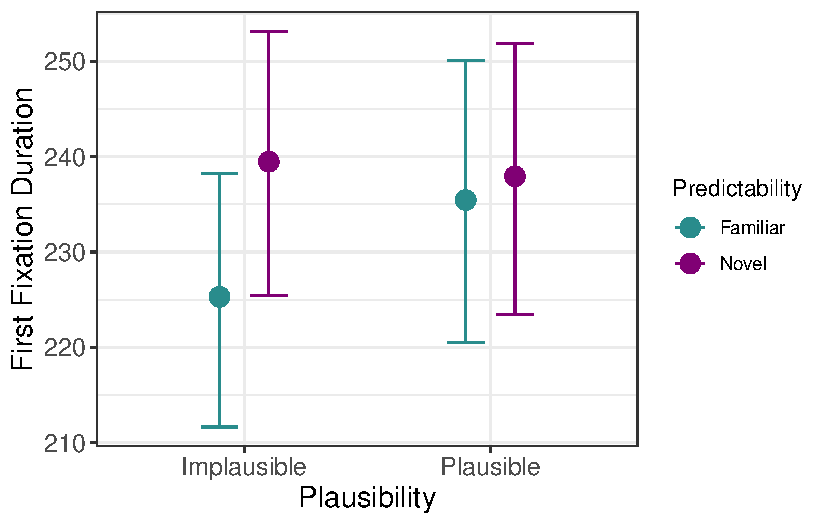
\includegraphics[width=0.8\textwidth,height=\textheight]{Chapters/Compound Nouns/staub_rep_ext_files/figure-pdf/fig-firstfixn2-1.pdf}

}

\caption{\label{fig-firstfixn2}Visualization of the effects of
plausibility and predictability on first fixation times for the N2
region.}

\end{figure}%

Unsurprisingly, our results demonstrate an effect of predictability on
the first fixation times of the second noun in the compound noun. This
is rather unsurprising because in the present study predictability is a
measure of how expected the second noun is given the first. There also
is not much of a plausibility effect on the N2, which is also not
particularly surprising because the second noun eliminates the local
implausibility. That is, both sentences are plausible at the N2 region.

\subsection{Gaze/First-Pass Time}\label{gazefirst-pass-time}

\subsubsection{N1}\label{n1-1}

Our results for the effects of plausibility and predictability on
gaze/first-pass times on the N1 region are presented in
\textbf{?@tbl-exp1m2} and visualized in \textbf{?@fig-exp1m2}.

\begin{longtable}[]{@{}
  >{\raggedright\arraybackslash}p{(\columnwidth - 10\tabcolsep) * \real{0.3636}}
  >{\raggedright\arraybackslash}p{(\columnwidth - 10\tabcolsep) * \real{0.1169}}
  >{\raggedright\arraybackslash}p{(\columnwidth - 10\tabcolsep) * \real{0.1299}}
  >{\raggedright\arraybackslash}p{(\columnwidth - 10\tabcolsep) * \real{0.1039}}
  >{\raggedright\arraybackslash}p{(\columnwidth - 10\tabcolsep) * \real{0.1039}}
  >{\raggedleft\arraybackslash}p{(\columnwidth - 10\tabcolsep) * \real{0.1818}}@{}}

\caption{\label{tbl-gazen1}Model results examining the effect of
plausibility and predictability on Gaze/first-pass times for the N1
region.}

\tabularnewline

\toprule\noalign{}
\begin{minipage}[b]{\linewidth}\raggedright
\end{minipage} & \begin{minipage}[b]{\linewidth}\raggedright
Estimate
\end{minipage} & \begin{minipage}[b]{\linewidth}\raggedright
Est.Error
\end{minipage} & \begin{minipage}[b]{\linewidth}\raggedright
Q2.5
\end{minipage} & \begin{minipage}[b]{\linewidth}\raggedright
Q97.5
\end{minipage} & \begin{minipage}[b]{\linewidth}\raggedleft
\% Samples \textgreater{} 0
\end{minipage} \\
\midrule\noalign{}
\endhead
\bottomrule\noalign{}
\endlastfoot
Intercept & 264.141 & 8.422 & 246.898 & 280.601 & 100.000 \\
Plausibility & -0.001 & 0.203 & -0.385 & 0.413 & 49.075 \\
Predictability & 0.005 & 0.198 & -0.394 & 0.387 & 51.475 \\
Plausibility:Predictability & -0.010 & 0.202 & -0.411 & 0.382 &
48.100 \\

\end{longtable}

\begin{figure}

\centering{

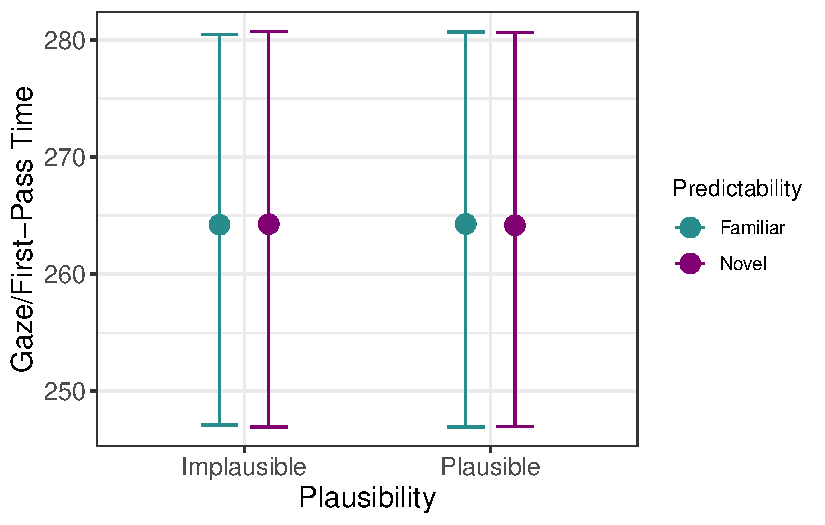
\includegraphics[width=0.8\textwidth,height=\textheight]{Chapters/Compound Nouns/staub_rep_ext_files/figure-pdf/fig-gazen1-1.pdf}

}

\caption{\label{fig-gazen1}Visualization of the effects of plausibility
and predictability on Gaze/first-pass times for the N1 region.}

\end{figure}%

Our results demonstrate no effect of either plausibility or
predictability on the gaze times at the N1 region. We further examined
our filler items to rule out an error with the eye-tracker. Our filler
items contain a frequency manipulation and an analysis of the filler
items demonstrated that the frequency manipulation did effect gaze times
in our filler items, suggesting that the results here are not due to any
malfunction of the eye-tracker or cleaning procedure.

\subsubsection{N2}\label{n2-1}

Our results for the N2 region are presented in Table~\ref{tbl-gazen2}
and visualized in Figure~\ref{fig-gazen2}.

\begin{longtable}[]{@{}
  >{\raggedright\arraybackslash}p{(\columnwidth - 10\tabcolsep) * \real{0.3636}}
  >{\raggedright\arraybackslash}p{(\columnwidth - 10\tabcolsep) * \real{0.1169}}
  >{\raggedright\arraybackslash}p{(\columnwidth - 10\tabcolsep) * \real{0.1299}}
  >{\raggedright\arraybackslash}p{(\columnwidth - 10\tabcolsep) * \real{0.1039}}
  >{\raggedright\arraybackslash}p{(\columnwidth - 10\tabcolsep) * \real{0.1039}}
  >{\raggedleft\arraybackslash}p{(\columnwidth - 10\tabcolsep) * \real{0.1818}}@{}}

\caption{\label{tbl-gazen2}Model results examining the effect of
plausibility and predictability on Gaze/first-pass times for the N2
region.}

\tabularnewline

\toprule\noalign{}
\begin{minipage}[b]{\linewidth}\raggedright
\end{minipage} & \begin{minipage}[b]{\linewidth}\raggedright
Estimate
\end{minipage} & \begin{minipage}[b]{\linewidth}\raggedright
Est.Error
\end{minipage} & \begin{minipage}[b]{\linewidth}\raggedright
Q2.5
\end{minipage} & \begin{minipage}[b]{\linewidth}\raggedright
Q97.5
\end{minipage} & \begin{minipage}[b]{\linewidth}\raggedleft
\% Samples \textgreater{} 0
\end{minipage} \\
\midrule\noalign{}
\endhead
\bottomrule\noalign{}
\endlastfoot
Intercept & 253.757 & 6.071 & 241.726 & 265.767 & 100.000 \\
Plausibility & -0.003 & 0.100 & -0.196 & 0.192 & 48.825 \\
Predictability & -0.003 & 0.101 & -0.207 & 0.190 & 48.625 \\
Plausibility:Predictability & 0.003 & 0.100 & -0.199 & 0.202 & 51.625 \\

\end{longtable}

\begin{figure}

\centering{

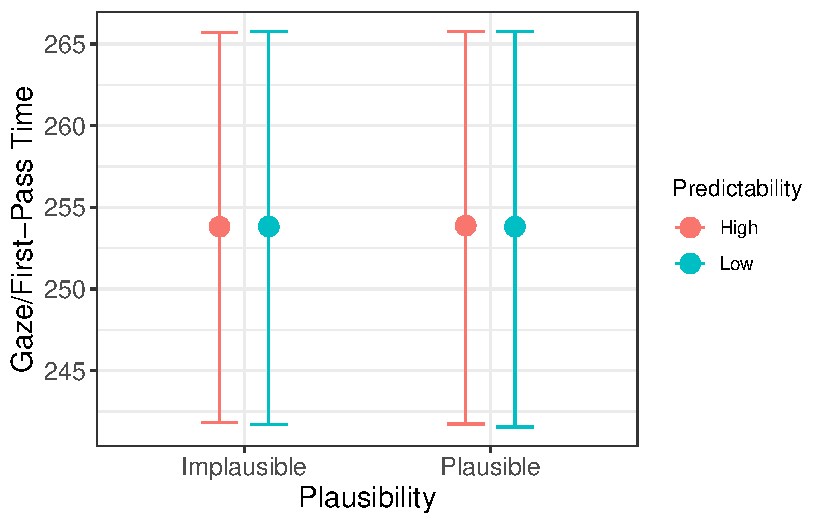
\includegraphics[width=0.8\textwidth,height=\textheight]{Chapters/Compound Nouns/staub_rep_ext_files/figure-pdf/fig-gazen2-1.pdf}

}

\caption{\label{fig-gazen2}Visualization of the effects of plausibility
and predictability on Gaze/first-pass times for the N2 region.}

\end{figure}%

The results of the N2 region also show a lack of effect of plausibility
and predictability on gaze times.

\subsection{Go-Past Time}\label{go-past-time}

\subsubsection{N1}\label{n1-2}

Our results for the effects of plausibility and predictability on
go-past times are presented in Table~\ref{tbl-gopastn1} and visualized
in Figure~\ref{fig-gopastn1}.

\begin{longtable}[]{@{}
  >{\raggedright\arraybackslash}p{(\columnwidth - 10\tabcolsep) * \real{0.3636}}
  >{\raggedright\arraybackslash}p{(\columnwidth - 10\tabcolsep) * \real{0.1169}}
  >{\raggedright\arraybackslash}p{(\columnwidth - 10\tabcolsep) * \real{0.1299}}
  >{\raggedright\arraybackslash}p{(\columnwidth - 10\tabcolsep) * \real{0.1039}}
  >{\raggedright\arraybackslash}p{(\columnwidth - 10\tabcolsep) * \real{0.1039}}
  >{\raggedleft\arraybackslash}p{(\columnwidth - 10\tabcolsep) * \real{0.1818}}@{}}

\caption{\label{tbl-gopastn1}Model results examining the effect of
plausibility and predictability on go-past times for the N1 region.}

\tabularnewline

\toprule\noalign{}
\begin{minipage}[b]{\linewidth}\raggedright
\end{minipage} & \begin{minipage}[b]{\linewidth}\raggedright
Estimate
\end{minipage} & \begin{minipage}[b]{\linewidth}\raggedright
Est.Error
\end{minipage} & \begin{minipage}[b]{\linewidth}\raggedright
Q2.5
\end{minipage} & \begin{minipage}[b]{\linewidth}\raggedright
Q97.5
\end{minipage} & \begin{minipage}[b]{\linewidth}\raggedleft
\% Samples \textgreater{} 0
\end{minipage} \\
\midrule\noalign{}
\endhead
\bottomrule\noalign{}
\endlastfoot
Intercept & 357.207 & 16.452 & 325.205 & 388.957 & 100.00000 \\
Plausibility & 0.018 & 0.197 & -0.367 & 0.400 & 54.05000 \\
Predictability & 0.005 & 0.200 & -0.390 & 0.394 & 50.10000 \\
Plausibility:Predictability & -0.000 & 0.200 & -0.392 & 0.393 &
49.76667 \\

\end{longtable}

\begin{figure}

\centering{

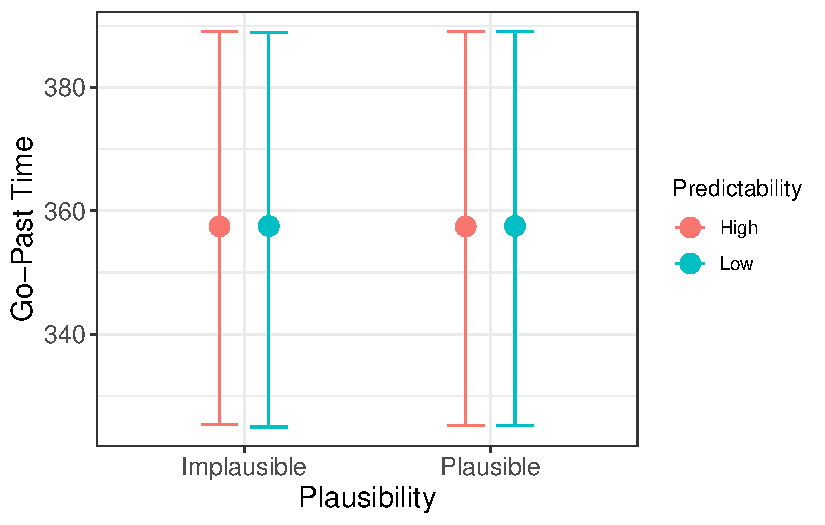
\includegraphics[width=0.8\textwidth,height=\textheight]{Chapters/Compound Nouns/staub_rep_ext_files/figure-pdf/fig-gopastn1-1.pdf}

}

\caption{\label{fig-gopastn1}Visualization of the effect of plausibility
and predictability on go-past times for the N1 region.}

\end{figure}%

Our results for go-past times similarly show no effect of predictability
and plausibility.

\subsubsection{N2}\label{n2-2}

Our results for the N2 region are presented in Table~\ref{tbl-gopastn2}
and visualized in Figure~\ref{fig-gopastn2}.

\begin{longtable}[]{@{}
  >{\raggedright\arraybackslash}p{(\columnwidth - 10\tabcolsep) * \real{0.3636}}
  >{\raggedright\arraybackslash}p{(\columnwidth - 10\tabcolsep) * \real{0.1169}}
  >{\raggedright\arraybackslash}p{(\columnwidth - 10\tabcolsep) * \real{0.1299}}
  >{\raggedright\arraybackslash}p{(\columnwidth - 10\tabcolsep) * \real{0.1039}}
  >{\raggedright\arraybackslash}p{(\columnwidth - 10\tabcolsep) * \real{0.1039}}
  >{\raggedleft\arraybackslash}p{(\columnwidth - 10\tabcolsep) * \real{0.1818}}@{}}

\caption{\label{tbl-gopastn2}Model results examining the effect of
plausibility and predictability on go-past times for the N2 region.}

\tabularnewline

\toprule\noalign{}
\begin{minipage}[b]{\linewidth}\raggedright
\end{minipage} & \begin{minipage}[b]{\linewidth}\raggedright
Estimate
\end{minipage} & \begin{minipage}[b]{\linewidth}\raggedright
Est.Error
\end{minipage} & \begin{minipage}[b]{\linewidth}\raggedright
Q2.5
\end{minipage} & \begin{minipage}[b]{\linewidth}\raggedright
Q97.5
\end{minipage} & \begin{minipage}[b]{\linewidth}\raggedleft
\% Samples \textgreater{} 0
\end{minipage} \\
\midrule\noalign{}
\endhead
\bottomrule\noalign{}
\endlastfoot
Intercept & 342.737 & 12.866 & 317.685 & 367.649 & 100.000 \\
Plausibility & -0.005 & 0.099 & -0.202 & 0.195 & 47.600 \\
Predictability & -0.001 & 0.100 & -0.198 & 0.195 & 50.000 \\
Plausibility:Predictability & -0.002 & 0.100 & -0.192 & 0.198 &
49.025 \\

\end{longtable}

\begin{figure}

\centering{

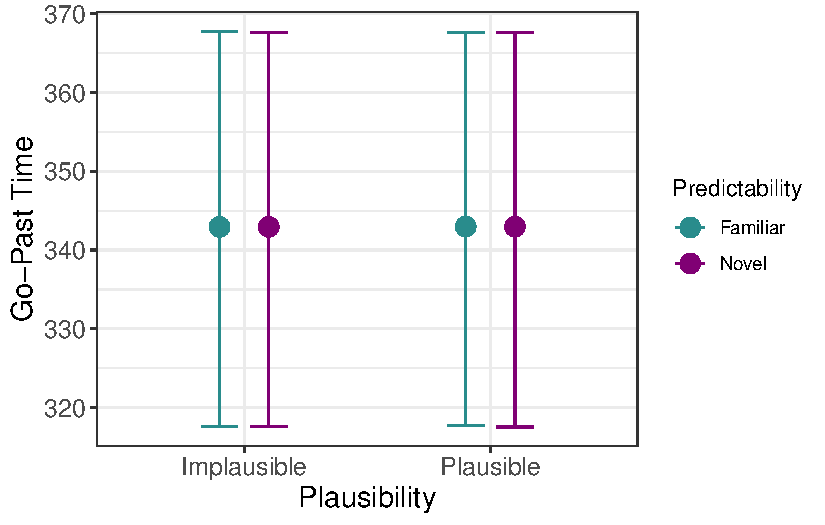
\includegraphics[width=0.8\textwidth,height=\textheight]{Chapters/Compound Nouns/staub_rep_ext_files/figure-pdf/fig-gopastn2-1.pdf}

}

\caption{\label{fig-gopastn2}Visualization of the effect of plausibility
and predictability on go-past times for the N2 region.}

\end{figure}%

Our results for the N2 region similarly show no effect of predictability
and plausibility on go-past times.

\subsection{First-Pass Regression}\label{first-pass-regression}

\subsubsection{N1}\label{n1-3}

Our results for the effects of predictability and plausibility on the
first-pass regression times on the N1 region are presented in
Table~\ref{tbl-firstpassn1} and visualized in
Figure~\ref{fig-firstpassn1}.

\begin{longtable}[]{@{}
  >{\raggedright\arraybackslash}p{(\columnwidth - 10\tabcolsep) * \real{0.3733}}
  >{\raggedright\arraybackslash}p{(\columnwidth - 10\tabcolsep) * \real{0.1200}}
  >{\raggedright\arraybackslash}p{(\columnwidth - 10\tabcolsep) * \real{0.1333}}
  >{\raggedright\arraybackslash}p{(\columnwidth - 10\tabcolsep) * \real{0.0933}}
  >{\raggedright\arraybackslash}p{(\columnwidth - 10\tabcolsep) * \real{0.0933}}
  >{\raggedleft\arraybackslash}p{(\columnwidth - 10\tabcolsep) * \real{0.1867}}@{}}

\caption{\label{tbl-firstpassn1}Model results examining the effect of
plausibility and predictability on first-pass regression for the N1
region.}

\tabularnewline

\toprule\noalign{}
\begin{minipage}[b]{\linewidth}\raggedright
\end{minipage} & \begin{minipage}[b]{\linewidth}\raggedright
Estimate
\end{minipage} & \begin{minipage}[b]{\linewidth}\raggedright
Est.Error
\end{minipage} & \begin{minipage}[b]{\linewidth}\raggedright
Q2.5
\end{minipage} & \begin{minipage}[b]{\linewidth}\raggedright
Q97.5
\end{minipage} & \begin{minipage}[b]{\linewidth}\raggedleft
\% Samples \textgreater{} 0
\end{minipage} \\
\midrule\noalign{}
\endhead
\bottomrule\noalign{}
\endlastfoot
Intercept & -1.645 & 0.151 & -1.948 & -1.358 & 0.000 \\
Plausibility & 0.199 & 0.080 & 0.041 & 0.357 & 99.375 \\
Predictability & -0.049 & 0.086 & -0.214 & 0.123 & 27.750 \\
Plausibility:Predictability & 0.128 & 0.075 & -0.019 & 0.275 & 96.025 \\

\end{longtable}

\begin{figure}

\centering{

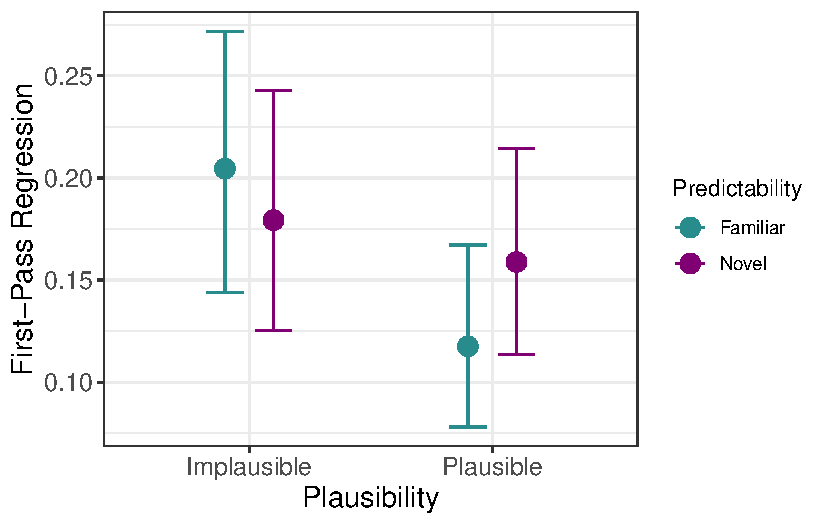
\includegraphics[width=0.8\textwidth,height=\textheight]{Chapters/Compound Nouns/staub_rep_ext_files/figure-pdf/fig-firstpassn1-1.pdf}

}

\caption{\label{fig-firstpassn1}Visualization of the effect of
plausibility and predictability on first-pass regression for the N1
region.}

\end{figure}%

Our results suggest that readers are more likely to regress after the
first fixation in the implausible condition compared to the plausible
condition. Further, this plausibility effect is larger for
high-predictability items than low predictability items. This is
surprising because predictability is a measure of the N2, not the N1 and
if readers are anticipating the N2 then it should alleviate the local
implausibility at the N1 (which would result in a negative interaction
effect, i.e.~the opposite trend from what we see here). Instead, we see
\ldots{}

\subsubsection{N2}\label{n2-3}

\begin{longtable}[]{@{}
  >{\raggedright\arraybackslash}p{(\columnwidth - 10\tabcolsep) * \real{0.3733}}
  >{\raggedright\arraybackslash}p{(\columnwidth - 10\tabcolsep) * \real{0.1200}}
  >{\raggedright\arraybackslash}p{(\columnwidth - 10\tabcolsep) * \real{0.1333}}
  >{\raggedright\arraybackslash}p{(\columnwidth - 10\tabcolsep) * \real{0.0933}}
  >{\raggedright\arraybackslash}p{(\columnwidth - 10\tabcolsep) * \real{0.0933}}
  >{\raggedleft\arraybackslash}p{(\columnwidth - 10\tabcolsep) * \real{0.1867}}@{}}

\caption{\label{tbl-firstpassn2}Model results examining the effect of
plausibility and predictability on first-pass regression for the N2
region.}

\tabularnewline

\toprule\noalign{}
\begin{minipage}[b]{\linewidth}\raggedright
\end{minipage} & \begin{minipage}[b]{\linewidth}\raggedright
Estimate
\end{minipage} & \begin{minipage}[b]{\linewidth}\raggedright
Est.Error
\end{minipage} & \begin{minipage}[b]{\linewidth}\raggedright
Q2.5
\end{minipage} & \begin{minipage}[b]{\linewidth}\raggedright
Q97.5
\end{minipage} & \begin{minipage}[b]{\linewidth}\raggedleft
\% Samples \textgreater{} 0
\end{minipage} \\
\midrule\noalign{}
\endhead
\bottomrule\noalign{}
\endlastfoot
Intercept & -2.061 & 0.176 & -2.426 & -1.728 & 0.000 \\
Plausibility & -0.026 & 0.106 & -0.241 & 0.184 & 40.625 \\
Predictability & -0.022 & 0.102 & -0.223 & 0.177 & 41.100 \\
Plausibility:Predictability & 0.049 & 0.097 & -0.136 & 0.239 & 69.975 \\

\end{longtable}

\begin{figure}

\centering{

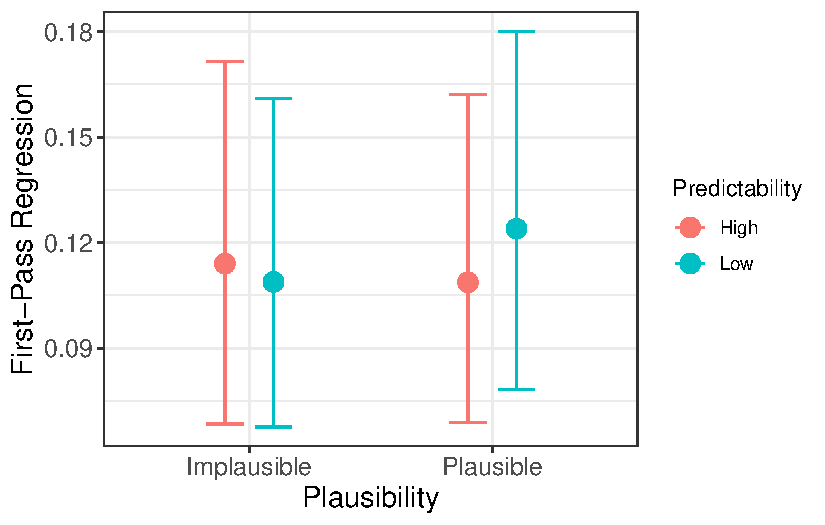
\includegraphics[width=0.8\textwidth,height=\textheight]{Chapters/Compound Nouns/staub_rep_ext_files/figure-pdf/fig-firstpassn2-1.pdf}

}

\caption{\label{fig-firstpassn2}Visualization of the effect of
plausibility and predictability on first-pass regression for the N2
region.}

\end{figure}%

Our results at the N2 region show no effect of predictability or
plausibility.

\section{Discussion}\label{discussion}

\bookmarksetup{startatroot}

\chapter*{References}\label{references}
\addcontentsline{toc}{chapter}{References}

\markboth{References}{References}

\phantomsection\label{refs}
\begin{CSLReferences}{1}{0}
\bibitem[\citeproctext]{ref-berkoChildsLearningEnglish1958}
Berko, Jean. 1958. {``The Child's Learning of English Morphology.''}
\emph{{\emph{WORD}}} 14 (2-3): 150--77.
\url{https://doi.org/10.1080/00437956.1958.11659661}.

\bibitem[\citeproctext]{ref-chomsky1965}
Chomsky, Noam. 1965. {``Aspects of the Theory of Syntax Special
Technical Report No. 11.''}
\url{https://ntrs.nasa.gov/api/citations/19670002070/downloads/19670002070.pdf}.

\bibitem[\citeproctext]{ref-houghtonTaskdependentConsequencesDisfluency2024}
Houghton, Zachary, Misaki Kato, Melissa Baese-Berk, and Charlotte
Vaughn. 2024. {``Task-Dependent Consequences of Disfluency in Perception
of Native and Non-Native Speech.''} \emph{Applied Psycholinguistics},
January, 1--17. \url{https://doi.org/10.1017/S0142716423000486}.

\bibitem[\citeproctext]{ref-kapatsinskiChangingMindsChanging2018}
Kapatsinski, Vsevolod. 2018. \emph{Changing Minds Changing Tools: From
Learning Theory to Language Acquisition to Language Change}. MIT Press.
\url{https://books.google.com/books?hl=en&lr=&id=YZxjDwAAQBAJ&oi=fnd&pg=PR5&dq=kapatsinski+changing+minds&ots=9bGhgkCaY0&sig=MHfWF9cbhbtMmx33a0FYSM6AMAs}.

\bibitem[\citeproctext]{ref-morganModelingIdiosyncraticPreferences2015}
Morgan, Emily, and Roger Levy. 2015. {``Modeling Idiosyncratic
Preferences : How Generative Knowledge and Expression Frequency Jointly
Determine Language Structure,''} 1649--54.

\bibitem[\citeproctext]{ref-morganAbstractKnowledgeDirect2016}
---------. 2016. {``Abstract Knowledge Versus Direct Experience in
Processing of Binomial Expressions.''} \emph{Cognition} 157: 384--402.
\url{https://doi.org/10.1016/j.cognition.2016.09.011}.

\bibitem[\citeproctext]{ref-staubTimeCoursePlausibility2007}
Staub, Adrian, Keith Rayner, Alexander Pollatsek, Jukka Hyönä, and Helen
Majewski. 2007. {``The Time Course of Plausibility Effects on Eye
Movements in Reading: Evidence from Noun-Noun Compounds.''}
\emph{Journal of Experimental Psychology: Learning Memory and Cognition}
33 (6): 1162--69. \url{https://doi.org/10.1037/0278-7393.33.6.1162}.

\bibitem[\citeproctext]{ref-stembergerFrequencyLexicalStorage1986}
Stemberger, Joseph Paul, and Brian MacWhinney. 1986. {``Frequency and
the Lexical Storage of Regularly Inflected Forms.''} \emph{Memory \&
Cognition} 14 (1): 17--26. \url{https://doi.org/10.3758/BF03209225}.

\bibitem[\citeproctext]{ref-stembergerAreInflectedForms2004}
Stemberger, Joseph P., and Brian MacWhinney. 2004. {``Are Inflected
Forms Stored in the Lexicon.''} \emph{Morphology: Critical Concepts in
Linguistics} 6: 107122.
\url{https://books.google.com/books?hl=en&lr=&id=bGl0aKBld3cC&oi=fnd&pg=PA107&dq=stemberger+2004+inflected&ots=RdvzVaC_NS&sig=0DJV8gUVaoZv_COZqcLXOu5_evU}.

\end{CSLReferences}




\end{document}
